%%%%%%%%%%%%%%%%%%%%%%%%%%%%%%%%%%%%%%%%%
% Beamer Presentation
% LaTeX Template
% Version 1.0 (10/11/12)
%
% This template has been downloaded from:
% http://www.LaTeXTemplates.com
%
% License:
% CC BY-NC-SA 3.0 (http://creativecommons.org/licenses/by-nc-sa/3.0/)
%
%%%%%%%%%%%%%%%%%%%%%%%%%%%%%%%%%%%%%%%%%

%----------------------------------------------------------------------------------------
% PACKAGES AND THEMES
%----------------------------------------------------------------------------------------

\documentclass[12pt,xcolor={dvipsnames}]{beamer}
%\setbeamersize{text margin left=1em,text margin right=1em}
\usepackage{mathtools}
\usepackage{amsmath}
\usepackage{bm}
\usepackage{hyperref}

\usepackage{graphicx} % Allows including images
\graphicspath{{/Users/rebecca/Documents/JER/MinimiseResponseMatrix/MCvsData/}{/Users/rebecca/Documents/Presentations/Talks/}}
\usepackage{booktabs} % Allows the use of \toprule, \midrule and \bottomrule in tables

\usepackage{etoolbox}

\usepackage{subcaption}
\captionsetup{compatibility=false}

\usepackage{multirow}

\usepackage{appendixnumberbeamer}

%\newlength\origleftmargini
%\setlength\origleftmargini\leftmargini
%\setbeamertemplate{itemize/enumerate body begin}{\setlength{\leftmargini}{2pt}}%

%\let\oldexampleblock\exampleblock
%\let\oldendexampleblock\endexampleblock
%\def\exampleblock{\begingroup \setbeamertemplate{itemize/enumerate body begin}{\setlength{\leftmargini}{\origleftmargini}} \oldexampleblock}
%\def\endexampleblock{\oldendexampleblock \endgroup}%

%\let\oldalertblock\alertblock
%\let\oldendalertblock\endalertblock
%\def\alertblock{\begingroup \setbeamertemplate{itemize/enumerate body begin}{\setlength{\leftmargini}{\origleftmargini}} \oldalertblock}
%\def\endalertblock{\oldendalertblock \endgroup}

\mode<presentation> {

% The Beamer class comes with a number of default slide themes
% which change the colors and layouts of slides. Below this is a list
% of all the themes, uncomment each in turn to see what they look like.

%\usetheme{default}
%\usetheme{AnnArbor}
%\usetheme{Antibes}
%\usetheme{Bergen}
%\usetheme{Berkeley}
%\usetheme{Berlin}
\usetheme{Boadilla}
%\usetheme{CambridgeUS}
%\usetheme{Copenhagen}
%\usetheme{Darmstadt}
%\usetheme{Dresden}
%\usetheme{Frankfurt}
%\usetheme{Goettingen}
%\usetheme{Hannover}
%\usetheme{Ilmenau}
%\usetheme{JuanLesPins}
%\usetheme{Luebeck}
%\usetheme{Madrid}
%\usetheme{Malmoe}
%\usetheme{Marburg}
%\usetheme{Montpellier}
%\usetheme{PaloAlto}
%\usetheme{Pittsburgh}
%\usetheme{Rochester}
%\usetheme{Seahorse}
%\usetheme{Singapore}
%\usetheme{Szeged}
%\usetheme{Warsaw}

% As well as themes, the Beamer class has a number of color themes
% for any slide theme. Uncomment each of these in turn to see how it
% changes the colors of your current slide theme.

%\usecolortheme{albatross}
%\usecolortheme{beaver}
%\usecolortheme{beetle}
%\usecolortheme{crane}
%\usecolortheme{dolphin}
%\usecolortheme{dove}
%\usecolortheme{fly}
%\usecolortheme{lily}
%\usecolortheme{RoyalBlue}
%\usecolortheme{rose}
%\usecolortheme{seagull}
%\usecolortheme{seahorse}
%\usecolortheme{whale}
%\usecolortheme{wolverine}

%%Changing the theme colours
%\setbeamercolor*{structure}{bg=Plum!20,fg=Plum}
%\setbeamercolor*{palette primary}{use=structure,fg=white,bg=structure.fg}
%\setbeamercolor*{palette secondary}{use=structure,fg=white,bg=structure.fg!75}
%\setbeamercolor*{palette tertiary}{use=structure,fg=white,bg=structure.fg!50!black}
%\setbeamercolor*{palette quaternary}{fg=white,bg=black}
%\setbeamercolor{section in toc}{fg=black,bg=white}
%%\setbeamercolor{alerted text}{use=structure,fg=structure.fg!50!black!80!black}
%\setbeamercolor{titlelike}{parent=palette primary,fg=structure.fg!50!black}
%\setbeamercolor{frametitle}{bg=gray!30!white,fg=Plum}
%\setbeamercolor*{titlelike}{parent=palette primary}

%Changing the theme colours
\setbeamercolor*{structure}{bg=RoyalPurple,fg=RoyalPurple}
\setbeamercolor*{palette primary}{use=structure,fg=white,bg=structure.fg}
\setbeamercolor*{palette secondary}{use=structure,fg=white,bg=structure.fg}
\setbeamercolor*{palette tertiary}{use=structure,fg=white,bg=structure.fg}
\setbeamercolor*{palette quaternary}{fg=white,bg=black}
\setbeamercolor{section in toc}{fg=black,bg=white}
%\setbeamercolor{alerted text}{use=structure,fg=structure.fg!50!black!80!black}
\setbeamercolor{titlelike}{parent=palette primary,fg=structure.fg!50!black}
%\setbeamercolor{frametitle}{use=structure,fg=white,bg=structure.fg}
\setbeamercolor*{titlelike}{parent=palette primary}

%\setbeamercolor{block}{bg=yellow!10,fg=black}
%\setbeamercolor{block title}{bg=yellow!50,fg=black}
%\AtBeginEnvironment{block}{\setbeamercolor{itemize item}{fg=yellow}}

\newenvironment<>{examplefirst}[1]{%
  \setbeamercolor{block title}{bg=yellow!50,fg=black}%
  \begin{block}#2{#1}}{\end{block}}
\AtBeginEnvironment{examplefirst}{\setbeamercolor{itemize item}{fg=yellow}}

%\setbeamertemplate{footline} % To remove the footer line in all slides uncomment this line
%\setbeamertemplate{footline}[page number] % To replace the footer line in all slides with a simple slide count uncomment this line

%\setbeamertemplate{navigation symbols}{} % To remove the navigation symbols from the bottom of all slides uncomment this line


\setbeamertemplate{blocks}[rounded][shadow=false]
\setbeamertemplate{itemize items}[circle]
\setbeamertemplate{itemize subitems}[circle]

\renewcommand{\thefootnote}{\alph{footnote}}

}

%----------------------------------------------------------------------------------------
% TITLE PAGE
%----------------------------------------------------------------------------------------



\title[Jet Energy Resolution Plots]{Jet Energy Resolution for the Dijet Balance Method} % The short title appears at the bottom of every slide, the full title is only on the title page

\author{\underline{Rebecca Pickles}} % Your name
%\institute[UoM] % Your institution as it will appear on the bottom of every slide, may be shorthand to save space
%{
%University of Manchester\\ % Your institution for the title page
%\medskip
%\textit{julia.iturbe@cern.ch} % Your email address
%}
% logo of my university
\titlegraphic{
\includegraphics[width=3cm]{UniOfManchesterLogo}}
\date{\today} % Date, can be changed to a custom date

\begin{document}


\begin{frame}
\titlepage % Print the title page as the first slide
\end{frame}

\iffalse
\begin{frame}
\frametitle{Overview} % Table of contents slide, comment this block out to remove it
\tableofcontents % Throughout your presentation, if you choose to use \section{} and \subsection{} commands, these will automatically be printed on this slide as an overview of your presentation
\end{frame}
\fi
%----------------------------------------------------------------------------------------
% PRESENTATION SLIDES
%----------------------------------------------------------------------------------------

%------------------------------------------------
\section{Introduction} % Sections can be created in order to organize your presentation into discrete blocks, all sections and subsections are automatically printed in the table of contents as an overview of the talk

%------------------------------------------------
\iffalse

\fi

\begin{frame}
\frametitle{Status}
\begin{itemize}
\item Produced plots of the fractional jet pT resolutions vs average pT and vs eta for:
\begin{itemize}
\item Data $\sqrt{s}$ = 13 TeV
\item Powheg+Pythia8 MC Reco 
\item Powheg+Pythia8 MC Truth
\end{itemize}
\end{itemize}
\end{frame}

\begin{frame}
\frametitle{JER vs Eta}
\begin{columns}
\begin{column}{.3\textwidth}
\includegraphics[width=4cm, height=3cm]{25pTavg40_MCvsData.pdf}
\newline
\includegraphics[width=4cm, height=3cm]{40pTavg55_MCvsData.pdf}
\end{column}
\begin{column}{.3\textwidth}
\includegraphics[width=4cm, height=3cm]{55pTavg70_MCvsData.pdf}
\newline
\includegraphics[width=4cm, height=3cm]{70pTavg85_MCvsData.pdf}
\end{column}
\begin{column}{.3\textwidth}
\includegraphics[width=4cm, height=3cm]{85pTavg115_MCvsData.pdf}
\newline
\includegraphics[width=4cm, height=3cm]{115pTavg145_MCvsData.pdf}
\end{column}
\end{columns}
\end{frame}

\begin{frame}
\frametitle{JER vs Eta: 25 $<$ pTavg $<$ 40}
\begin{columns}
\begin{column}{.3\textwidth}
\vspace{2.9cm}
\center{Data}
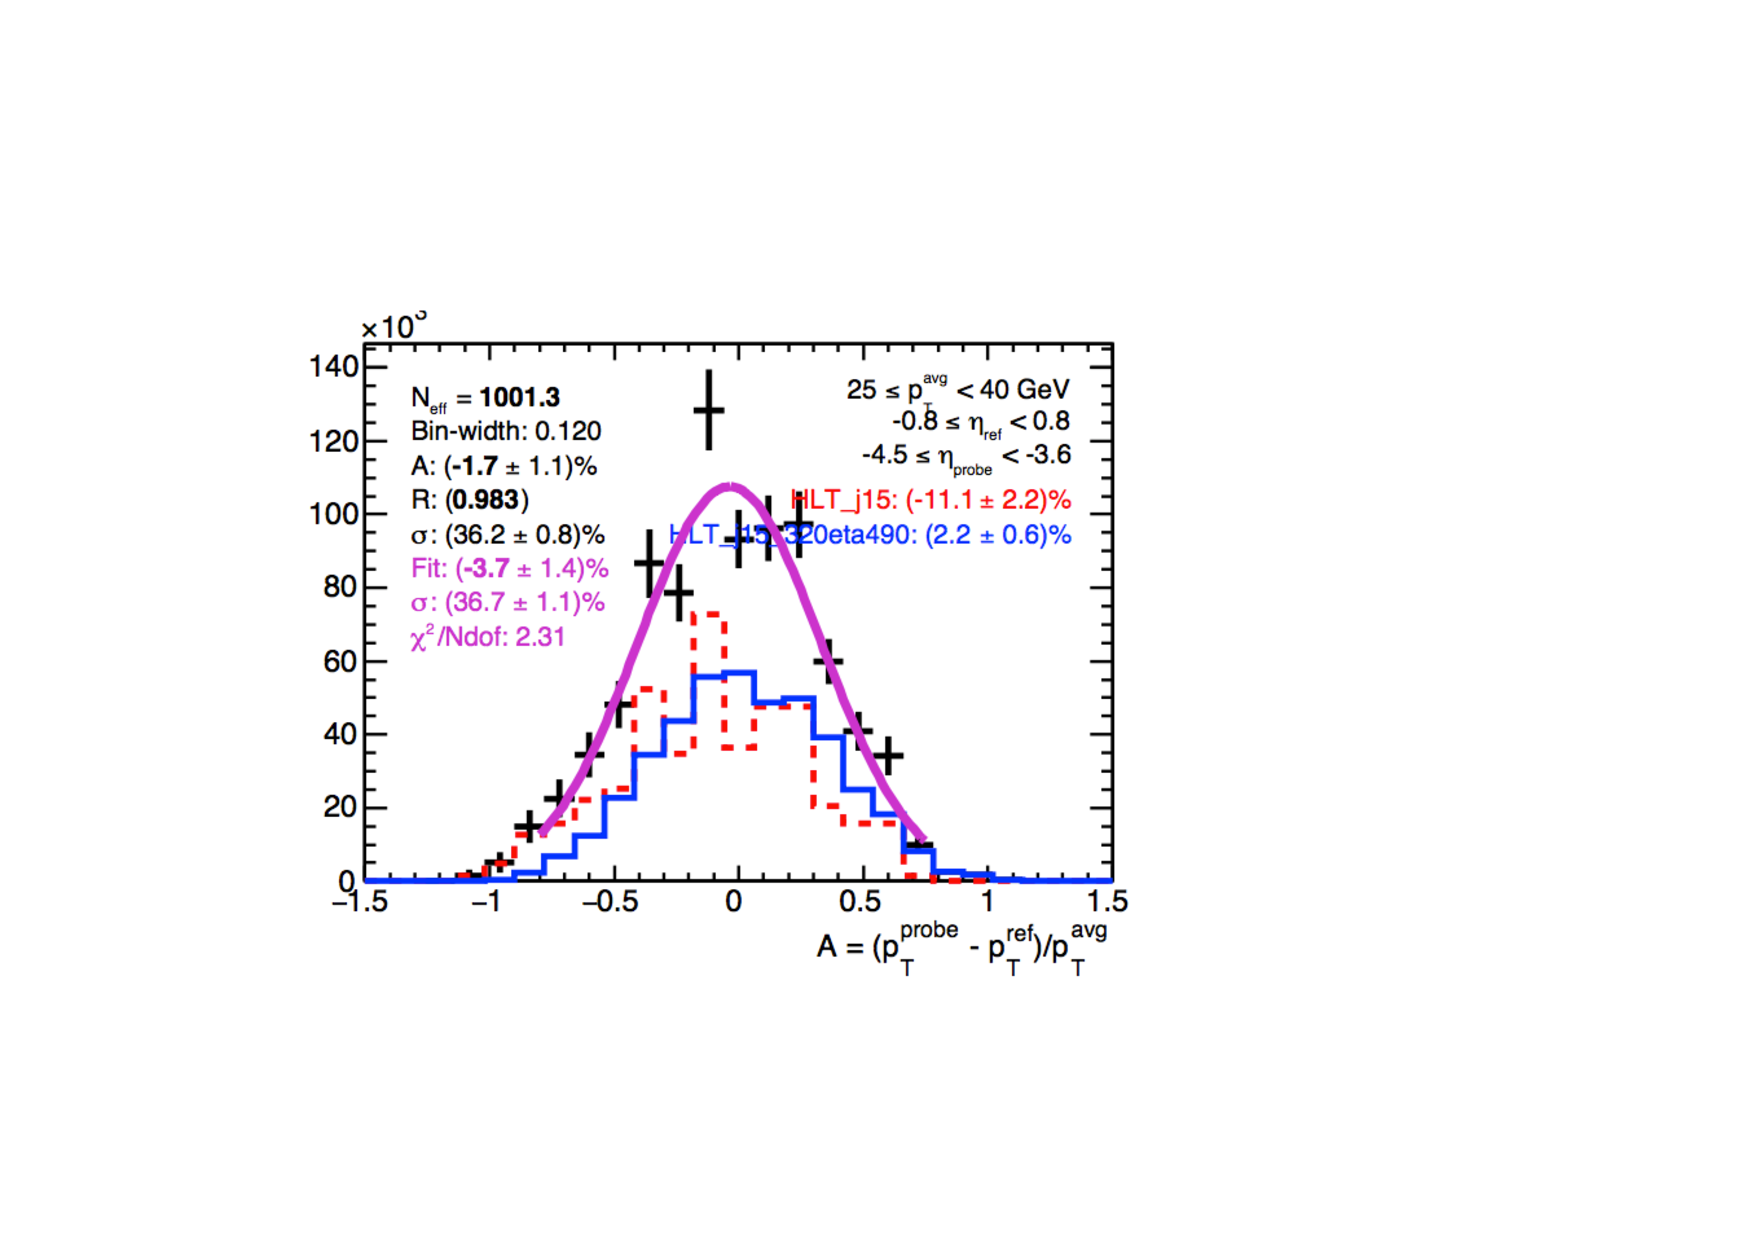
\includegraphics[width=4cm, height=3cm]{JER_fit_25to40_Data.pdf}
\end{column}
\begin{column}{.3\textwidth}
\includegraphics[width=4cm, height=3cm]{25pTavg40_MCvsData.pdf}
\center{MC EMTopo}
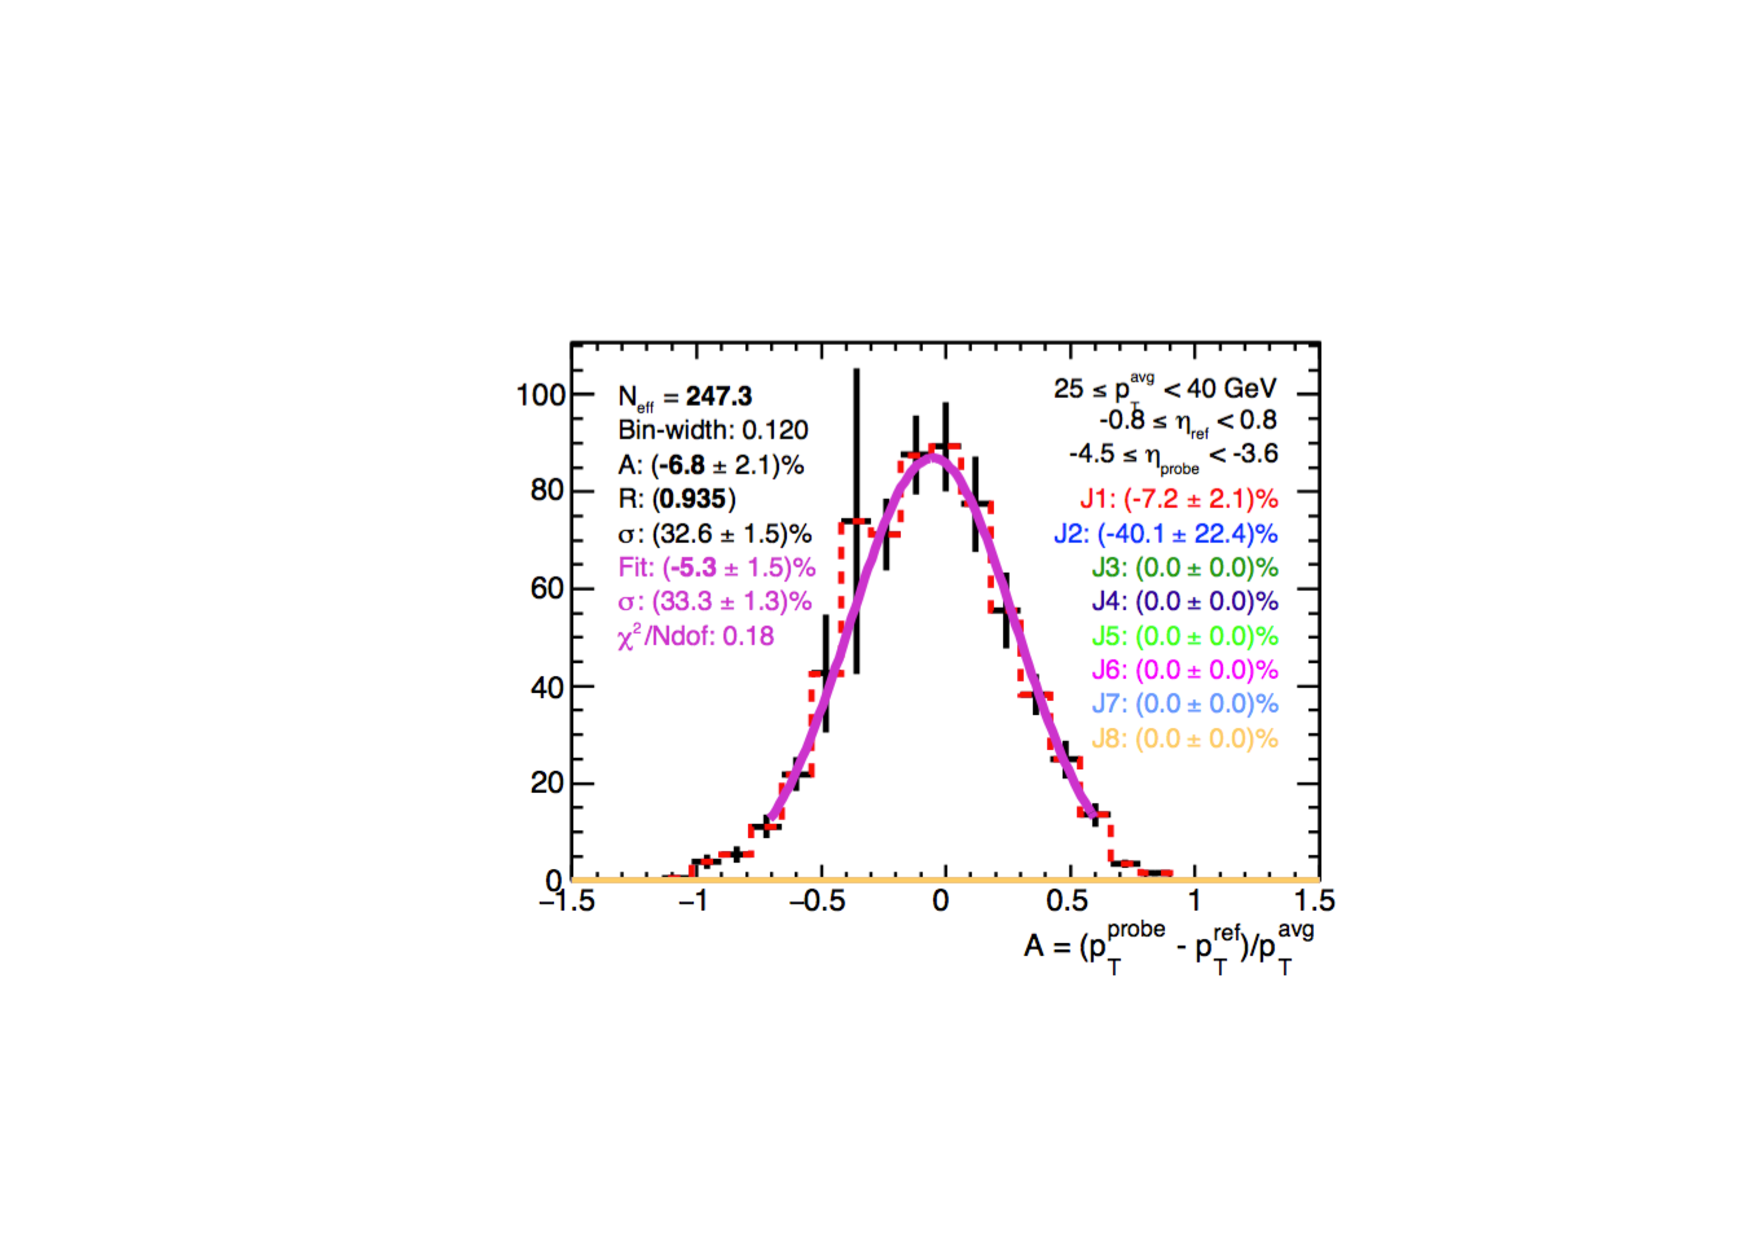
\includegraphics[width=4cm, height=3cm]{JER_fit_25to40_EMTopo.pdf}
\end{column}
\begin{column}{.3\textwidth}
\vspace{2.9cm}
\center{MC Truth}
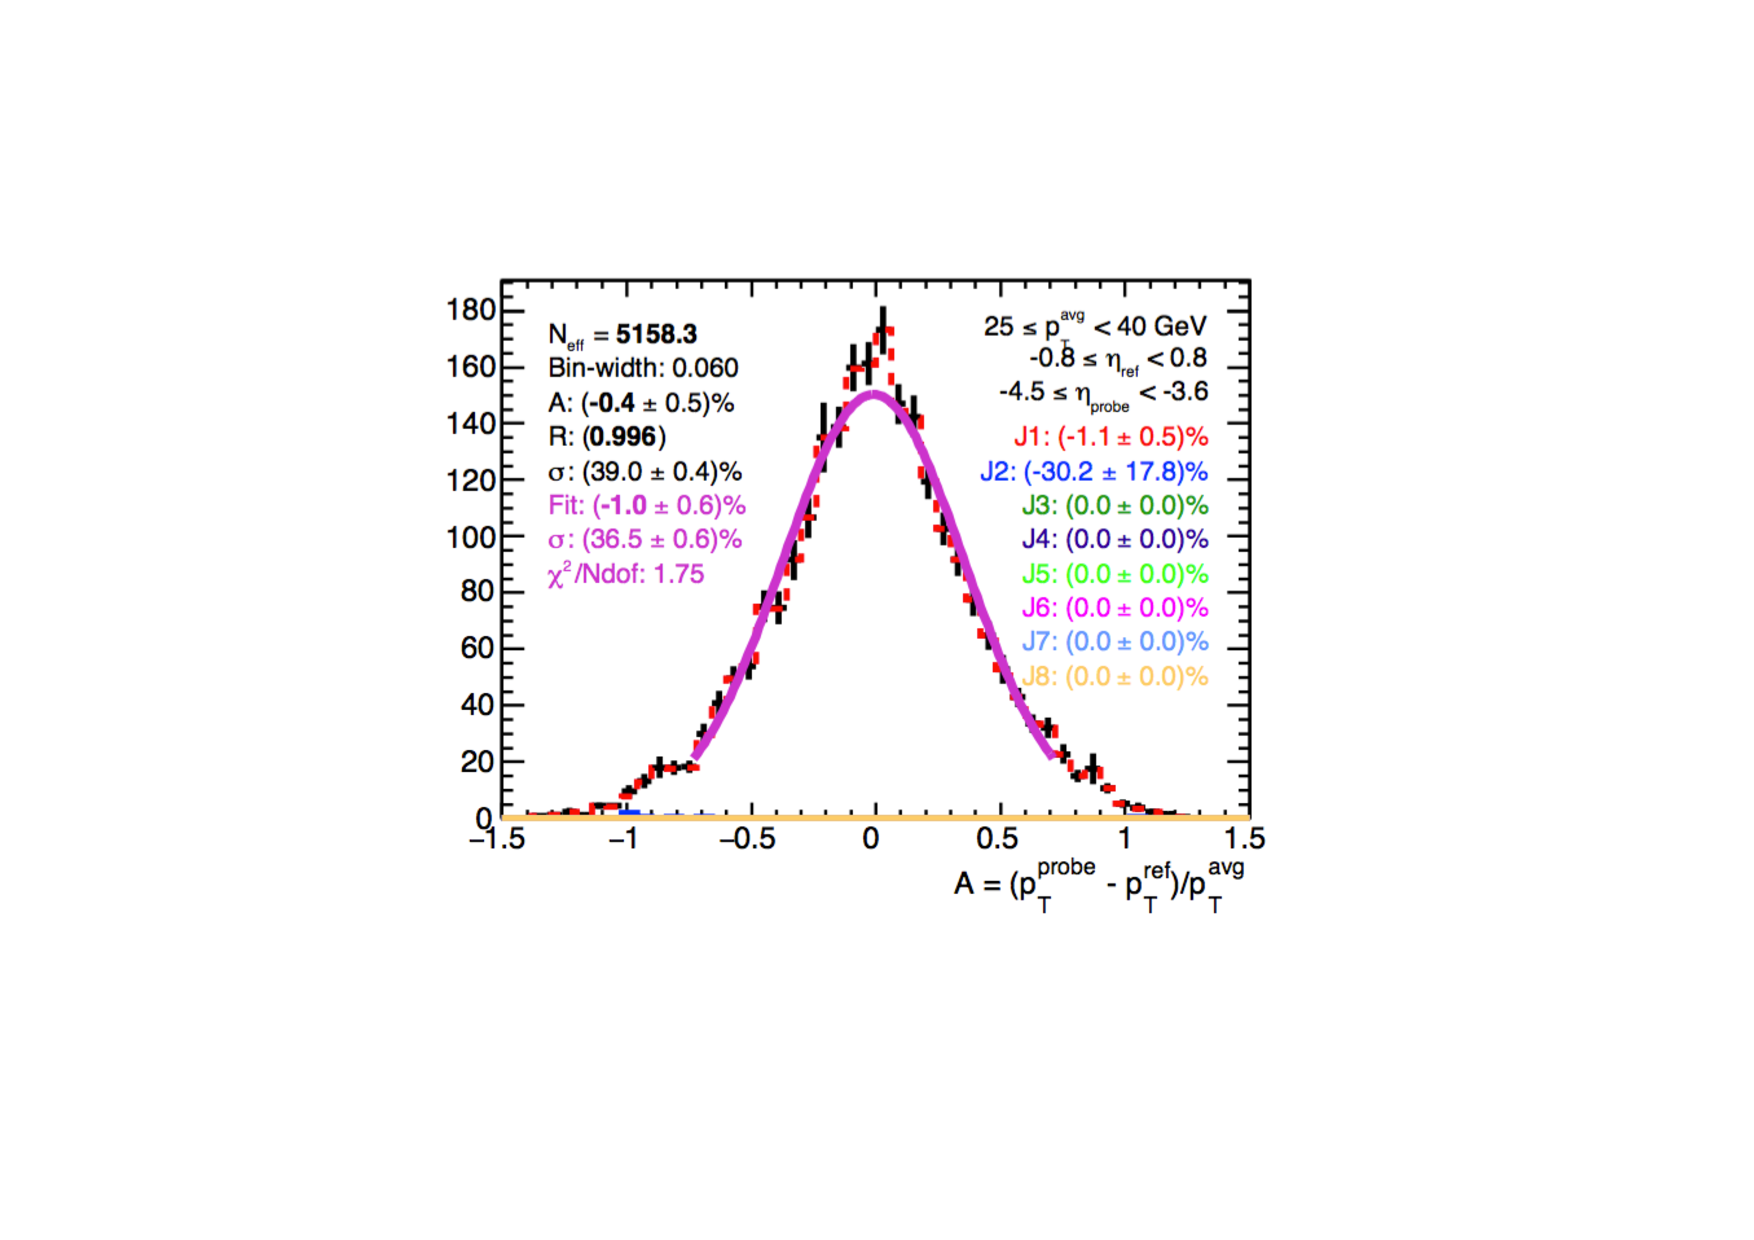
\includegraphics[width=4cm, height=3cm]{JER_fit_25to40_Truth.pdf}
\end{column}
\end{columns}
\end{frame}

\begin{frame}
\frametitle{JER vs Eta}
\begin{columns}
\begin{column}{.3\textwidth}
\includegraphics[width=4cm, height=3cm]{145pTavg175_MCvsData.pdf}
\newline
\includegraphics[width=4cm, height=3cm]{175pTavg220_MCvsData.pdf}
\end{column}
\begin{column}{.3\textwidth}
\includegraphics[width=4cm, height=3cm]{220pTavg270_MCvsData.pdf}
\newline
\includegraphics[width=4cm, height=3cm]{270pTavg330_MCvsData.pdf}
\end{column}
\begin{column}{.3\textwidth}
\includegraphics[width=4cm, height=3cm]{400pTavg525_MCvsData.pdf}
\newline
\includegraphics[width=4cm, height=3cm]{760pTavg1200_MCvsData.pdf}
\end{column}
\end{columns}
\end{frame}

\begin{frame}
\frametitle{Problems with the fit}
\begin{columns}
\begin{column}{.5\textwidth}
\includegraphics[width=6cm, height=4cm]{330pTavg400_MCvsData.pdf}
\newline
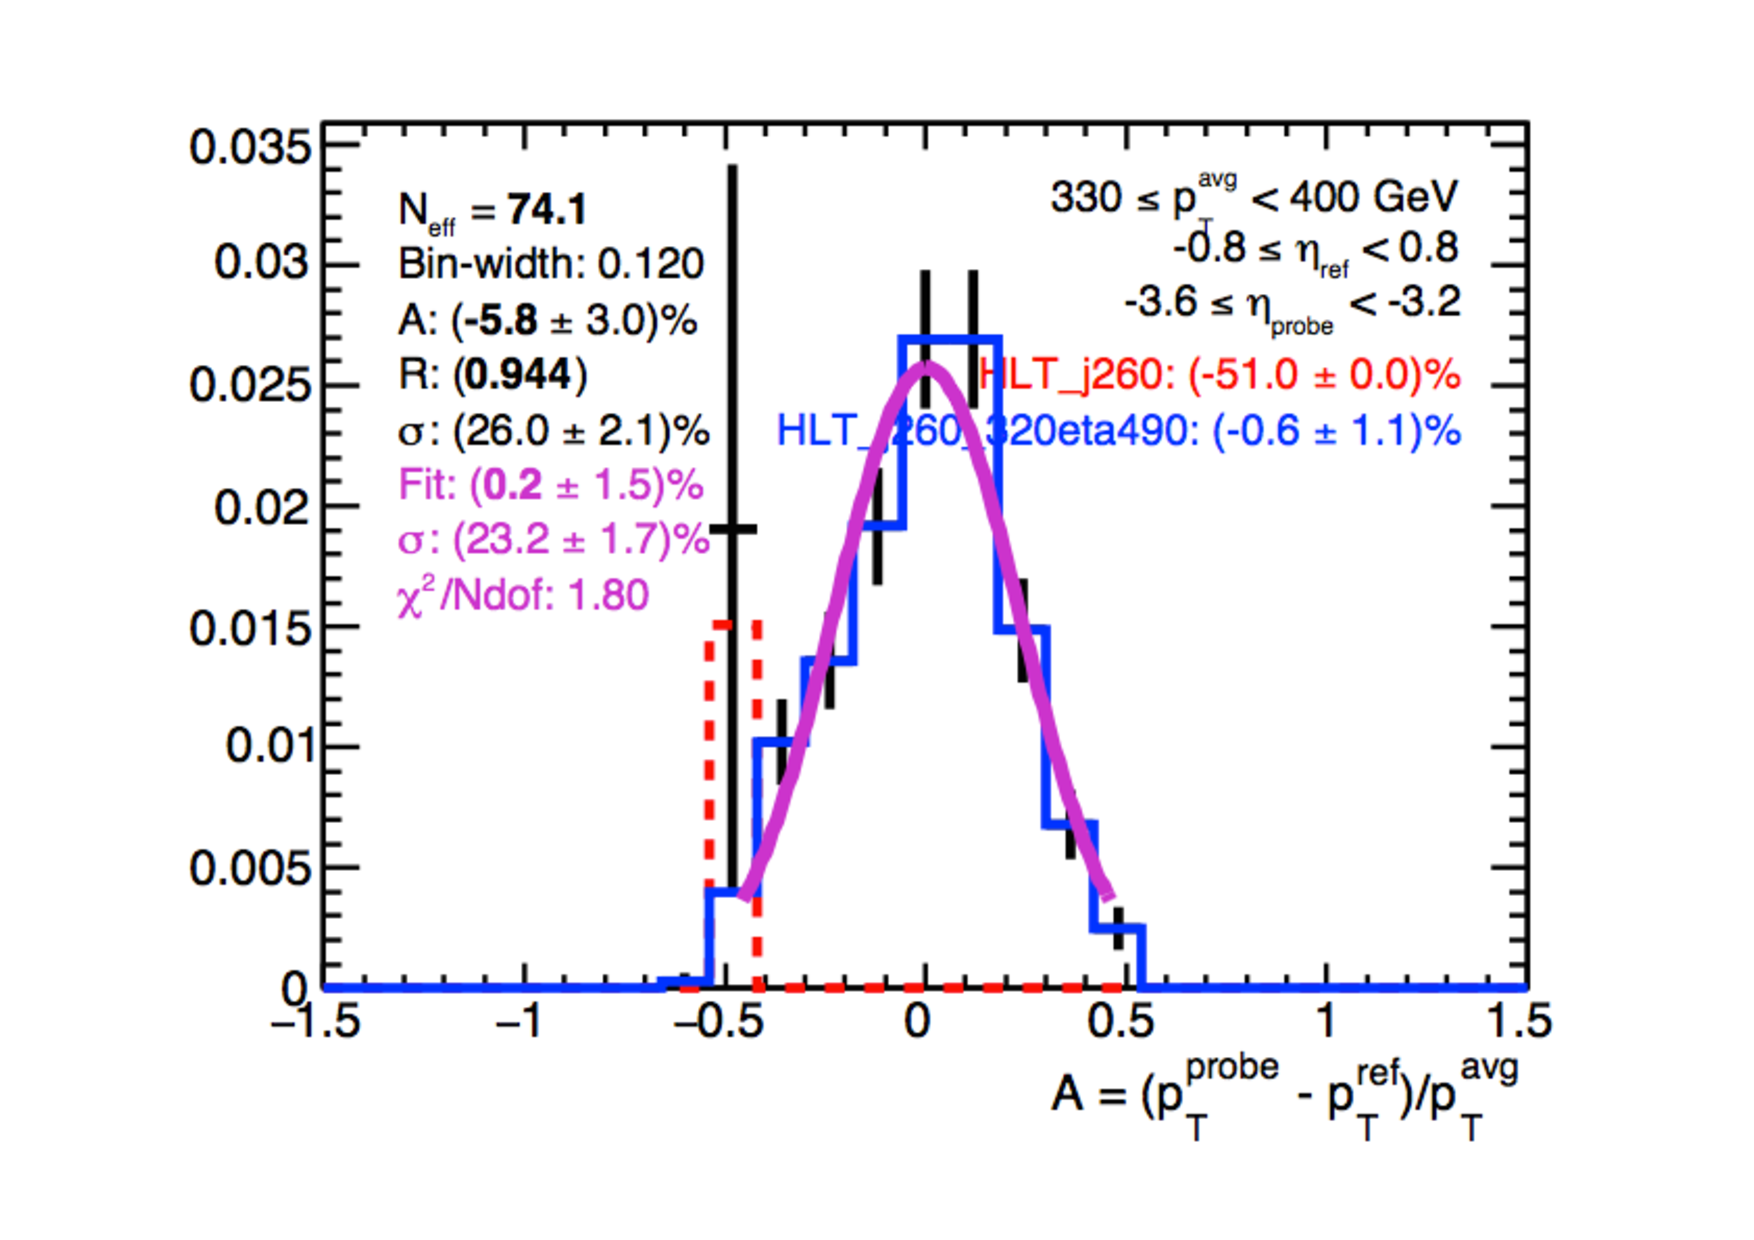
\includegraphics[width=6cm, height=4cm]{JER_fit_330to400.pdf}
\end{column}
\begin{column}{.5\textwidth}
\includegraphics[width=6cm, height=4cm]{525pTavg760_MCvsData.pdf}
\newline
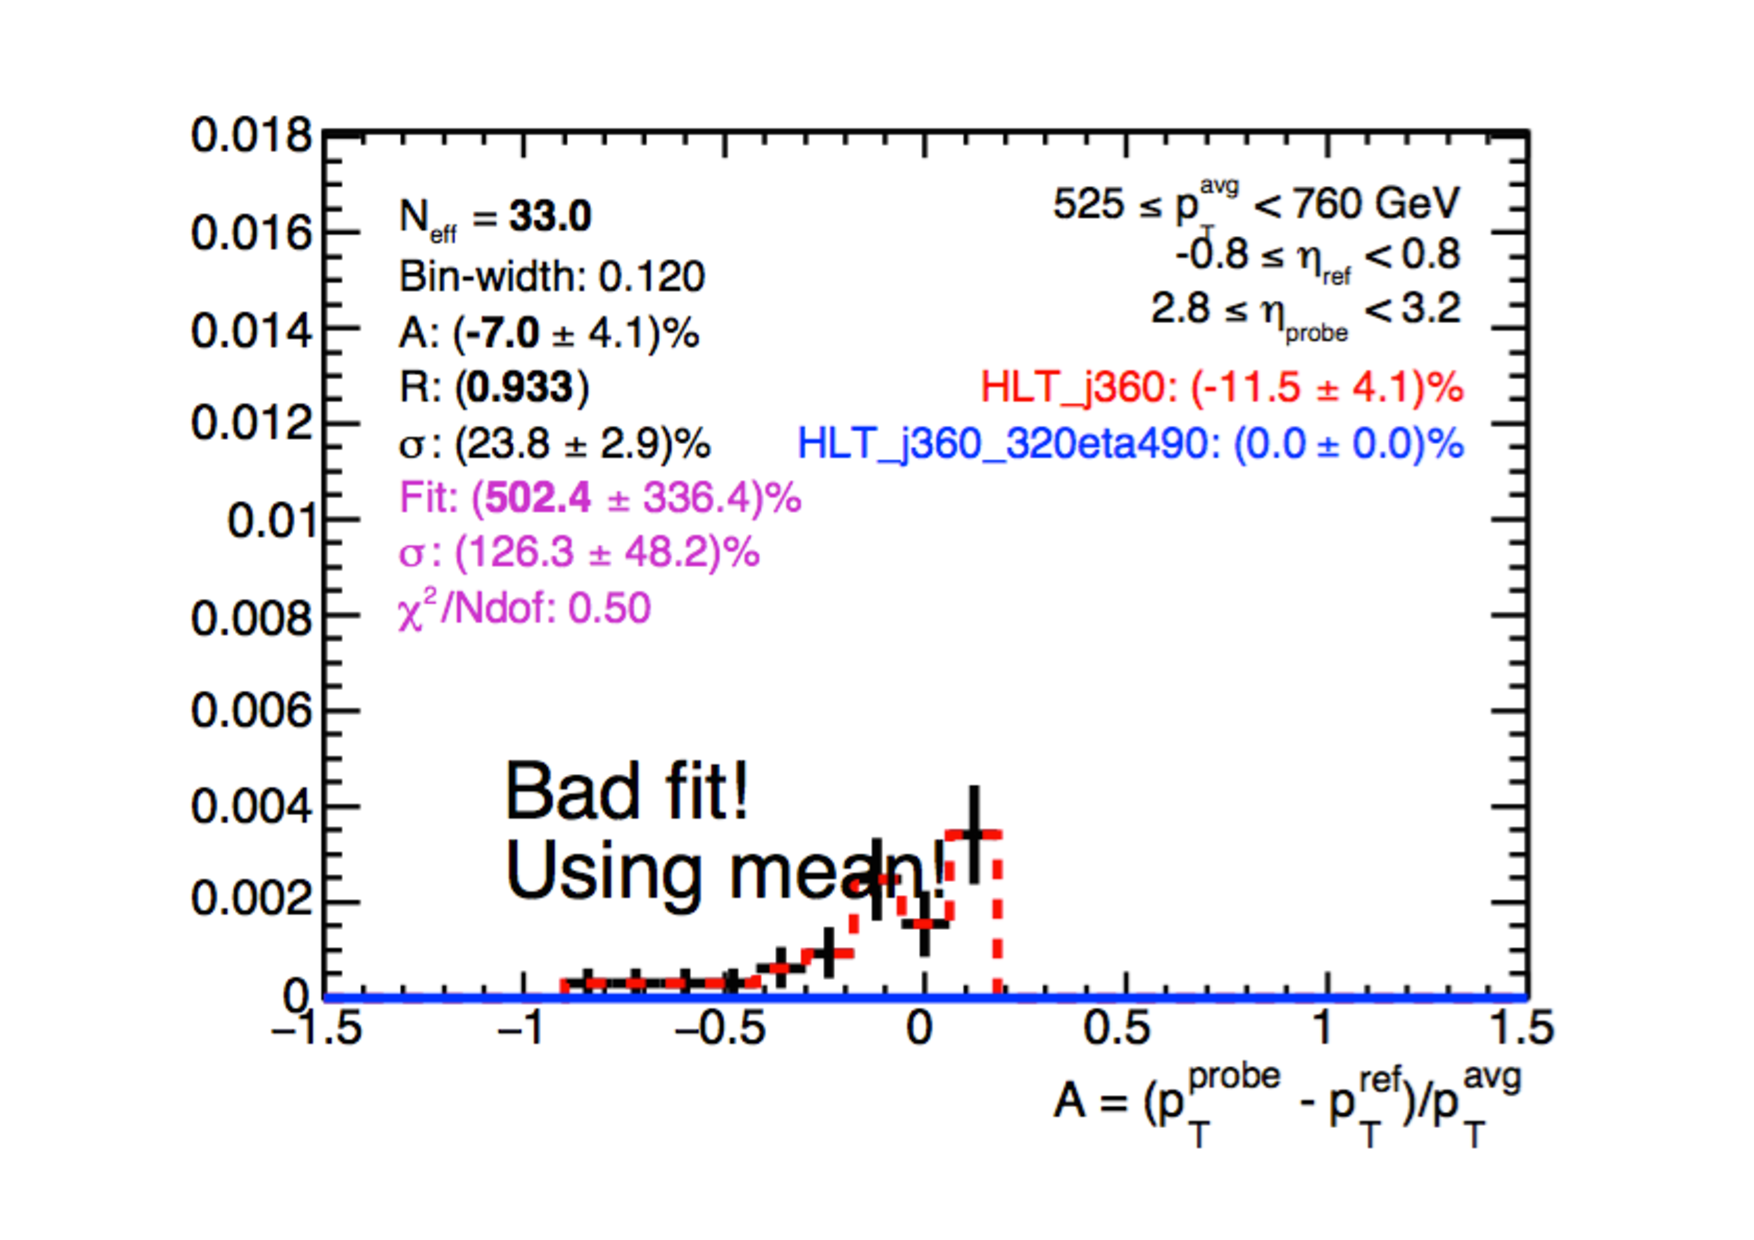
\includegraphics[width=6cm, height=4cm]{JER_fit_525to760.pdf}
\end{column}
\end{columns}
\end{frame}

\begin{frame}
\frametitle{JER vs pT}
\begin{columns}
\begin{column}{.3\textwidth}
\includegraphics[width=4cm, height=3cm]{etaBin4_MCvsData.pdf}
\newline
\includegraphics[width=4cm, height=3cm]{etaBin5_MCvsData.pdf}
\end{column}
\begin{column}{.3\textwidth}
\includegraphics[width=4cm, height=3cm]{etaBin6_MCvsData.pdf}
\newline
\includegraphics[width=4cm, height=3cm]{etaBin7_MCvsData.pdf}
\end{column}
\begin{column}{.3\textwidth}
\includegraphics[width=4cm, height=3cm]{etaBin8_MCvsData.pdf}
\newline
\includegraphics[width=4cm, height=3cm]{etaBin9_MCvsData.pdf}
\end{column}
\end{columns}
\end{frame}

\begin{frame}
\frametitle{JER vs pT}
\begin{columns}
\begin{column}{.3\textwidth}
\includegraphics[width=4cm, height=3cm]{etaBin10_MCvsData.pdf}
\newline
\includegraphics[width=4cm, height=3cm]{etaBin11_MCvsData.pdf}
\end{column}
\begin{column}{.3\textwidth}
\includegraphics[width=4cm, height=3cm]{etaBin12_MCvsData.pdf}
\newline
\includegraphics[width=4cm, height=3cm]{etaBin13_MCvsData.pdf}
\end{column}
\begin{column}{.3\textwidth}
\includegraphics[width=4cm, height=3cm]{etaBin14_MCvsData.pdf}
\newline
\includegraphics[width=4cm, height=3cm]{etaBin15_MCvsData.pdf}
\end{column}
\end{columns}
\end{frame}

\begin{frame}
\frametitle{Next Steps:}
\begin{itemize}
\item Subtract the true (physics) resolution from the reco
\item Study systematically varied MC subtractions
\item Extract a mean resolution and compare with the MC simulated resolution and other systematic studies
\item Any suggestions for other studies?
\end{itemize}
\end{frame}




\end{document} 